\chapter{How to Speak}

This lecture treats speaking as a craft with structure, technique, and consequences. It does not begin with tips. It begins with urgency, then narrows that urgency into a formula for communicative quality, and only after that does it unfold the machinery: how to start, how to keep people from drifting away, how to use boards and props, why slides so often fail, what a job talk must establish almost at once, and how a speaker should stop. The order is pedagogical. We are first persuaded that there is something to know, and then shown what that knowledge looks like in practice.

\section{Opening Hook, Communication Formula, and the Promise}

Winston opens with a forceful analogy. The Uniform Code of Military Justice, he says, punishes an officer who sends a soldier into battle without a weapon. There ought to be an analogous protection for students, because students should not be sent into life without the ability to communicate. The point is not literary refinement. The point is that ideas do not travel on their own.

He then states the ranking as bluntly as one could wish:

\begin{equation}
\text{speaking} \succ \text{writing} \succ \text{quality of ideas}.
\end{equation}

Here \(\succ\) is only editorial shorthand for his phrase ``in that order.'' The claim is not that ideas are intrinsically less important than delivery, but that success in the world is often filtered by the order in which these things fail or succeed.

From there the lecture narrows to its first formal object. Using the secure transcript lines rather than the later blackboard residue, we may write the opening formula in the cautious standard form

\begin{equation}
Q = f(K,P,T),
\end{equation}

where \(Q\) denotes the quality of speaking or writing, \(K\) is knowledge, \(P\) is practice, and \(T\) is inherent talent.

\begin{remark}
The later classroom frame with the bicycle wheel still shows only a partial background residue of this formula, namely something like \(\text{Quality}=f(K,P,\ldots)\). The full three-variable form is therefore reconstructed here from the transcript, not transcribed completely from the screenshot alone.
\end{remark}

The lecture immediately tells us how to read the formula. It is not symmetric in its arguments. Winston says that the \(T\) is ``very small.'' In compact mathematical shorthand, not as his own board notation but as a faithful summary of his meaning, we may write

\begin{equation}
T \ll K,P.
\end{equation}

The key word is not merely ``practice,'' but ``knowledge.'' Winston says very explicitly: what really matters is what you know.

He then tests the formula with a story rather than an argument in the abstract. Mary Lou Retton is an extraordinary athlete, but she is a novice skier. Winston is much less gifted athletically, yet a better skier. Why? Because on that problem he has the relevant \(K\) and \(P\), while she mainly has \(T\). The anecdote is not decoration around the formula. It is the first proof that the formula should be taken seriously.

\subsection{Question \& Answer}

\paragraph{Question.} Why is \(T\) small?

\paragraph{Answer.} Because talent by itself is not yet task-specific competence. The skiing example makes the point as sharply as possible. Retton has immense general athletic talent, but Winston has skiing knowledge and skiing practice. So on skis he is better. The lecture wants us to transfer that structure directly to speaking. A person with moderate native gifts and strong models, habits, and preparation can outstrip a more naturally gifted but less trained speaker.

From the anecdote the lecture moves at once to promise. If the formula is right, then improvement is not mysterious. The audience is promised an armamentarium of speaking techniques, and Winston adds an important rider: the process is nonlinear. Perhaps one of those techniques, maybe only one, will be the one that gets someone the job. This is not a throwaway line. It is the motivational bridge from theory to the rest of the hour.

\section{Rules of Engagement and How to Start}

Only after making that promise does Winston impose discipline. The no-laptops and no-cellphones rule is not presented as a matter of decorum. It is presented as a fact about cognition. Human beings, he says, have one language processor. If that processor is reading email or browsing the web, then it is not listening. Worse, the damage is social: surrounding listeners are distracted, and the speaker performs worse when open laptops remain in view.

This is one of the lecture's governing ideas. It will return later as the deepest argument against text-heavy slides. Here it performs a different function. It clears the channel before the lecture proper begins.

The next move is equally deliberate. ``First thing to talk about,'' Winston says, ``is how to start.'' He immediately rejects a familiar piece of advice: beginning with a joke. The reason is not that jokes are beneath serious speaking. The reason is timing. Early in the talk the room is still adjusting to the speaker's voice, pace, and rhythm. The audience is not yet synchronized.

\subsection{Question \& Answer}

\paragraph{Question.} Why not start with a joke?

\paragraph{Answer.} Because a joke requires a settled audience, and the beginning of a talk gives us an unsettled one. People are still arriving, still putting things away, still adjusting to the speaker's vocal parameters. A joke therefore comes before the audience is ready to receive it. What belongs at the beginning instead is an empowerment promise: a clear statement of what the audience will know at the end of the hour that they do not know at the beginning.

This is one of the lecture's nicest reflexive features. Winston is not only recommending the empowerment promise; he is already carrying one out. The lecture has opened with urgency, then a formula, then an anecdotal proof, and now a promise of usable techniques. The talk is already being used as its own example.

\section{The Four Heuristics}

Once the audience has been persuaded that there is real knowledge here, Winston gives four sample heuristics that are always on his mind when he speaks: cycle on the subject, build a fence around the idea, use verbal punctuation, and ask a question.

\paragraph{Cycle.} The first heuristic is to go around the subject, and then go around it again. Winston recalls the old advice: tell them what you are going to tell them, tell them, and then tell them a third time. His justification is not that listeners are dull. It is that listeners are intermittent. At any given moment, he says, about \(20\%\) of the room is fogged out no matter what the lecture is.

That heuristic invites a small editorial model. If \(p_{\mathrm{fog}}\) denotes the chance that a listener misses a given pass, then Winston's \(20\%\) estimate gives

\begin{align}
p_{\mathrm{fog}} &\approx 0.2,\\
\mathrm{Prob}(\text{miss all three passes}) &\approx p_{\mathrm{fog}}^3 = 0.2^3 = 0.008,\\
\mathrm{Prob}(\text{catch at least one pass}) &\approx 1-p_{\mathrm{fog}}^3 = 0.992.
\end{align}

\begin{remark}
This is our explanatory gloss, not Winston's own calculation. The lecture's real point is practical rather than probabilistic: repetition creates multiple opportunities for re-entry.
\end{remark}

\subsection{Question \& Answer}

\paragraph{Question.} Why say it three times?

\paragraph{Answer.} Because speaking happens in time, and audiences do not hold perfectly still. A single pass is fragile. A second and third pass, especially when they approach the same point from slightly different sides, make the communication robust. ``Cycle'' is therefore not empty redundancy. It is an engineering response to drifting attention.

\paragraph{Build a fence.} The second heuristic is definitional by contrast. If we want an audience to know what our idea is, we should also help them see what it is not. Winston's simple example is the arch: this is an arch; this is not an arch; that is not an arch. The technical form is equally useful: my algorithm resembles Jones's algorithm, except that his is exponential and mine is linear. A concept acquires sharpness when we build a fence around it.

\paragraph{Verbal punctuation.} The third heuristic comes from the same diagnosis of attention. If people fall off the bus, they need seams in the talk where they can get back on. Explicit enumeration, recap, and transition phrases provide those seams. Winston's own lecture demonstrates the method as he moves from the first idea to the second and then announces that he is now on the third.

\paragraph{Ask a question.} The fourth heuristic is the most direct re-engagement device. A question interrupts passive reception and makes the room orient itself toward a problem. But here too the lecture adds a measured rule. One must wait long enough.

\begin{equation}
t_{\mathrm{wait}} \approx 7\,\mathrm{s}.
\end{equation}

Seven seconds feels like an eternity to the speaker. That is precisely why the rule is needed. The room requires thinking time. At the same time, the question must be chosen carefully: not so obvious that answering feels embarrassing, and not so difficult that nobody can say anything.

At the end of this block Winston pauses to say something revealing. If the audience is now persuaded that there is ``something to know'' about speaking, then he has already succeeded. That is the hinge on which the lecture turns. Only now does he broaden the frame.

\section{Time and Place as Part of the Argument}

The next thing on the agenda, Winston says, is time and place. The transition is explicit, and the lecture wants us to feel that the widening is earned. First we dealt with the inner mechanics of a talk; now we consider the conditions under which those mechanics can work.

The preferred lecture time is \(11\) a.m. Winston's reasons are practical and bodily: people are awake, not just after a meal, and not yet dropping into fatigue. The preferred room is well lit, because dim rooms signal sleep. It should also be cased in advance, which is to say inspected beforehand so that live surprises are minimized. Finally, it should be reasonably populated. A half-empty hall produces its own discouraging social theater.

These points survive visually in one of the lecture's best blackboard frames. The screenshot is valuable not because it contains a derivation, but because it preserves the board's architecture.

\begin{figure}[h]
\centering

\includegraphics[width=0.95\textwidth]{lecture_11_figure_03.png}
\end{figure}

The left side is headed \emph{Samples} and lists the four heuristics. The loop beside ``Cycle'' is not a formal diagram, but it is a useful visual encoding of the repeated-pass idea. The right side is headed \emph{Time \& Place}, separated by a long wavy stroke. The blackboard is already doing what Winston says a good board should do: organize a talk spatially, not merely verbally.

A cleaned reconstruction makes that organization easier to read. The exact right-hand wording is not fully secure from the frame alone, so the items below are completed from the transcript while preserving the board's overall geometry.

\begin{figure}[h]
\centering
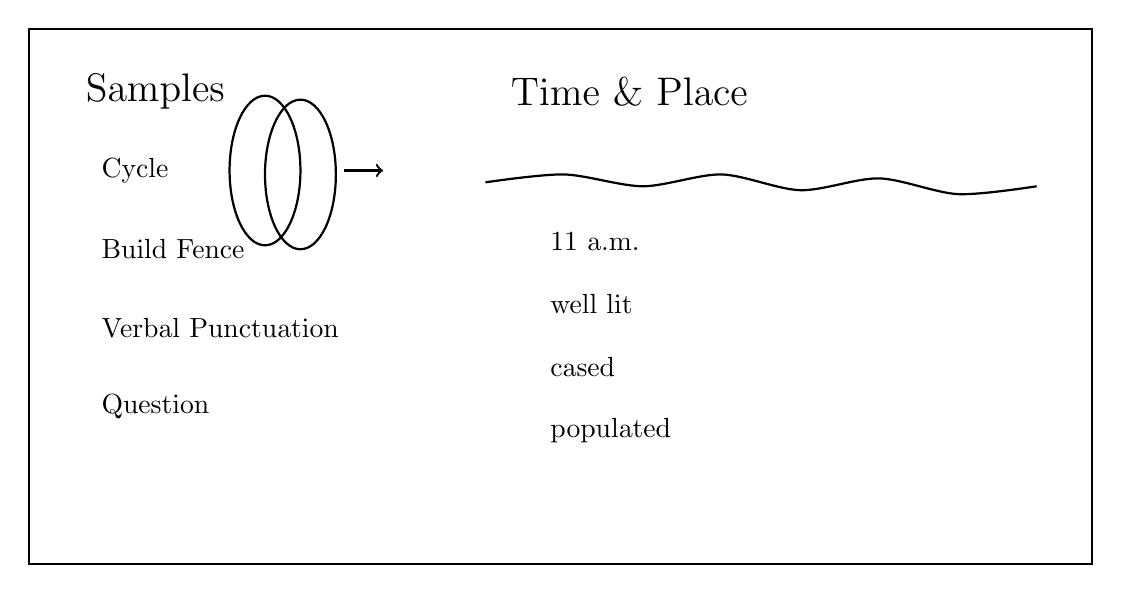
\begin{tikzpicture}[x=1cm,y=1cm]
\draw[thick] (0,0) rectangle (13.5,6.8);

\node[anchor=west] at (0.6,6.0) {\Large Samples};
\node[anchor=west] at (0.8,5.0) {Cycle};
\draw[thick] (3.0,5.0) ellipse (0.45 and 0.95);
\draw[thick] (3.45,4.95) ellipse (0.45 and 0.95);
\draw[->,thick] (4.0,5.0) -- (4.5,5.0);

\node[anchor=west] at (0.8,4.0) {Build Fence};
\node[anchor=west] at (0.8,3.0) {Verbal Punctuation};
\node[anchor=west] at (0.8,2.0) {Question};

\node[anchor=west] at (6.0,6.0) {\Large Time \& Place};
\draw[thick] plot[smooth] coordinates {(5.8,4.85) (6.8,4.95) (7.8,4.8) (8.8,4.95) (9.8,4.75) (10.8,4.9) (11.8,4.7) (12.8,4.8)};
\node[anchor=west] at (6.5,4.1) {11 a.m.};
\node[anchor=west] at (6.5,3.3) {well lit};
\node[anchor=west] at (6.5,2.5) {cased};
\node[anchor=west] at (6.5,1.7) {populated};
\end{tikzpicture}
\end{figure}

What the lecture is really saying is that time and place are not merely logistical details. They are variables in the dynamics of attention.

\section{Boards and Props: Why Physical Media Work}

Only after time and place does Winston move to tools. The order is important. A tool is not chosen in a vacuum; it is chosen inside a room, at a time, for a purpose.

The basic distinction is simple. A board is the right tool when the aim is informing, teaching, or lecturing. Slides are better suited to exposing ideas quickly, as in conference talks and job talks. Winston then gives three reasons for preferring the board in genuine teaching.

First, it has graphic quality. A board lets us group, separate, underline, and sketch. Second, it has a speed property: the speed of writing is roughly the speed at which an audience can absorb. Slides can outrun thought. Third, the board provides a target for the speaker's hands. This is more than a joke. Much awkwardness in public speaking comes from a sudden self-consciousness about the body, and the board gives that body honest work to do.

From here the lecture broadens to props. The guiding principle is once again example before theory. Ibsen's stove in \emph{Hedda Gabler} works because it sits there, gathers tension, and slowly becomes inevitable. The prop is memorable because it is not merely described; it is staged.

That same logic appears in the classroom. Papert's bicycle wheel is not decoration. It is a device for carrying a line of reasoning.

\begin{figure}[h]
\centering

\includegraphics[width=0.78\textwidth]{lecture_11_figure_04.png}
\end{figure}

The figure is important primarily for the physical demonstration: the wheel is upright, the hub is in the lecturer's hands, and the prop is fully visible. In the background one can still see a partial residue of the opening blackboard formula, something like \(\text{Quality}=f(K,P,\ldots)\), together with the earlier stove sketch. But the mathematical burden of the figure lies with the prop, not with those remnants.

\subsection{Question \& Answer}

\paragraph{Question.} Which way does the spinning wheel go?

\paragraph{Answer.} Winston's point is that memorized hand rules are a poor way to think about this demonstration. He says, rhetorically, that many mechanical engineers wind up at about a \(50\%\) success rate, which means that the rule has become equivalent to a coin toss. The better method is to change the representation of the problem.

\begin{enumerate}
\item Start the wheel spinning and mark a small rim segment with duct tape.
\item Refuse, for the moment, to think about the wheel as a whole.
\item Watch the marked segment come over the top.
\item Apply the puff of air, or the effective local push, to that segment.
\item Ask what that one small piece now wants to do.
\item Then watch the next piece arrive in the same position.
\item The same local reasoning applies again.
\item Therefore the wheel as a whole must continue in the corresponding direction.
\end{enumerate}

The achievement here is not a full gyroscopic analysis. The lecture never writes one, and we should not import it as though it had been present. The achievement is pedagogical. The prop permits a local-piece argument that replaces memorized symbolism with a more reliable picture.

The second prop example is Alan Lazarus's pendulum ball demonstration of conservation of energy. A heavy ball is lifted to nose height, released from rest, swings away, and then returns to kiss but not destroy the demonstrator's nose. The relevant equation is the canonical one:

\begin{equation}
E = K_{\mathrm{kin}} + V_{\mathrm{pot}} = \text{const.}
\end{equation}

The lecture does not derive this on the board, and it does not need to. The point is that the demonstration makes the law bodily memorable. The real danger, Winston says, is not the failure of conservation but the human tendency to push instead of simply letting go.

Only after the stove, the wheel, and the pendulum does Winston offer a general explanation. Chalk and props, he says in his ``lunatic fringe'' theory, work because of empathetic mirroring. When we watch a hand write, or a ball swing, we almost feel ourselves writing or swinging. A slide or picture does not produce the same embodied participation. Once again the lecture keeps faith with its own method: example first, explanation second.

\section{Slides, Special Cases, and the Job Talk Threshold}

There is, Winston says, one more tool to discuss: slides. The distinction from earlier is repeated with more force now that the board and props have been established. Slides are for exposing ideas, not for teaching them.

The attack begins with a law stated as if it hardly admits exceptions: people always have too many slides, and those slides always have too many words. From there the lecture becomes a catalog of slide crimes. One must not read the slide aloud. One must not stand so far from it that the audience is forced into a visual tennis match between screen and speaker. One should strip away background junk, gratuitous logos, and titles that the speaker is already saying aloud.

The deeper argument is the same one-language-processor claim from the beginning. Dense slides recruit the audience into reading, and once the room is reading it is not listening. Winston reinforces the point with an experiment: when part of the content is spoken and part appears on the slide, students remember the slide content better. One of them later says that the speaker's talking was distracting. The joke lands because the principle is true.

The lecture then sharpens the advice. A slide should usually carry only a few words. If there is historical text that matters, the speaker should explicitly give the audience time to read it. And there is one interesting exception: Winston's \emph{hapax legomenon} slide, the impossibly dense slide that is allowable exactly once when the whole point is to display complexity itself. But once means once.

Typographically the rule is practical:

\begin{equation}
40\text{--}50\,\mathrm{pt}\ \text{is safe}, \qquad 35\,\mathrm{pt}\ \text{is already drifting too small.}
\end{equation}

The lecture's point is not just that \(35\) point may be hard to read. It is that speakers reach for \(35\) point when they are trying to get too much language onto the slide.

Winston adds further crimes: the laser pointer, which forces the speaker to turn away from the audience; the too-heavy deck, which can be diagnosed by printing the slides and laying them all out on a table; the deck with no air, no white space, and no imagery. The cumulative lesson is that slides should be condiments to the spoken line of reasoning, not a rival lecture happening on the wall.

From tools the lecture moves into special cases. The first is informing, which is to say the kind of speaking Winston is doing right now. Here the empowerment promise returns, but with a new emphasis: to inspire, one must do more than structure information. One may tell students they can do it, help them see a problem in a new way, or simply exhibit genuine passion for the subject. The resource-allocation story is his example. First we are shown a catastrophic brute-force computation; then we are promised that a small change, explained over the next fifty minutes, will collapse a lifetime-of-the-solar-system computation into seconds. The promise is both explanatory and thrilling.

Then comes a smaller digression on what faculty often say they do: teach people how to think. Winston asks the next question that such a claim invites: how? His answer is that we are storytelling animals. To teach thought is therefore to provide stories, questions about stories, mechanisms for analysis, ways of putting stories together, and ways of evaluating their reliability. This digression matters because it connects presentation not just to persuasion but to education.

Oral exams then supply two more pieces of advice. A candidate must situate the work, meaning place it in the larger field and explain why the problem matters. And practice must be real practice, not rehearsal in front of people who already know the material and silently fill in missing explanations.

\subsection{Question \& Answer}

\paragraph{Question.} How long do you have in a job talk?

\paragraph{Answer.} About five minutes.

\begin{equation}
t_{\mathrm{job}} \approx 5\,\mathrm{min}.
\end{equation}

Within that window, Winston says, two things must be established. The audience must see that the candidate has vision, and it must also see that the candidate has done something. Vision means a problem someone cares about together with something genuinely new in the approach. ``Done something'' means that there is concrete progress, not just aspiration.

The lecture makes this concrete by recommendation. The speaker should enumerate the steps required to solve the problem, show which of those steps have actually been carried out, and then mirror those steps at the end in a contributions slide. A compact technical-talk structure therefore emerges:

\begin{enumerate}
\item state the problem worth caring about,
\item identify what is new in the approach,
\item list the steps that would be required for real progress,
\item show that some of those steps have in fact been achieved,
\item conclude with a contributions slide that mirrors the earlier list.
\end{enumerate}

This is more than etiquette. It is a theory of how a stranger decides, very quickly, whether a speaker has a research program rather than a collection of isolated facts.

\section{Getting Remembered and Knowing How to Stop}

The lecture's last movement begins after the job talk. Once the job is obtained, Winston says, one still has to think about being recognized for the value of the work. He stages this with the Julia Child anecdote. People keep approaching her to say that she changed their lives. Her answer to whether it is fun to be famous is dry: one gets used to it. Winston's reply is more revealing: one never gets used to being ignored. The moral is that packaging is not vanity. It is part of giving ideas a fair chance in the world.

From there he introduces Winston's Star, the five-part structure by which work becomes memorable:

\begin{itemize}
\item symbol,
\item slogan,
\item surprise,
\item salient idea,
\item story.
\end{itemize}

The old arch-learning example unfolds the star. The arch itself is the symbol. ``One-shot learning'' is the slogan. The surprise is that one example can teach something definite if the learner is clever enough. The salient idea is the near miss: not merely a negative example, but an almost-example that reveals what the concept really requires. And then everything must be tied together into a story of how the system works and why it matters. Winston stresses that ``salient'' here does not mean ``important'' in the abstract. It means the idea that sticks out enough to remain in memory.

Only after memory comes closure. The lecture now stages bad endings. One should not end with a huge list of collaborators, because that shrinks the speaker just when the audience is deciding what the speaker has done. One should not waste the last screen on empty space. One should not end with ``conclusions'' if what really matters is contribution.

\subsection{Question \& Answer}

\paragraph{Question.} What should the final slide and final words do?

\paragraph{Answer.} The final slide should display contributions, and the final words should perform a real closing gesture rather than a weak act of politeness.

The last slide remains visible while people ask questions and while they leave the room. It should therefore keep the strongest compression of the work in view. ``Contributions'' is Winston's preferred label precisely because it mirrors the earlier list of what had to be done and of what has in fact been done.

The final words are a separate art. A joke can work at the end, Winston says, because by then the audience has adjusted to the speaker and can receive the timing. But he does not recommend ending with ``thank you'' as the main concluding move. Such an ending suggests that the audience has remained from courtesy rather than because the talk was worth hearing. He therefore looks elsewhere for examples: political benedictions, ceremonial dismissal formulas, concert conventions, and finally the gesture he most wants to recommend here, namely a salute to the audience and the place.

This too is enacted by the lecture itself. Winston tells the audience that by being present they have already demonstrated an understanding that presentation matters, and he salutes them for it. Only after the real closing gesture comes a final polite thank-you. The order matters.

\section{Summary}

The lecture proceeds by deliberate narrowing and widening. It narrows first to a formula,
\[
Q=f(K,P,T),
\]
and then immediately breaks the symmetry of that formula by shrinking \(T\). It widens into heuristics, then into the room, then into the choice of medium, then into special cases such as oral exams and job talks, and finally narrows again into compact summary devices: Winston's Star, the contributions slide, and the closing gesture.

What unifies the whole lecture is a single practical question: how do we give ideas the maximum chance of surviving contact with time, distraction, embodiment, and memory? Winston's answer is not one trick. It is a repertoire. We motivate, we promise, we cycle, we fence, we punctuate, we ask, we choose the room, we choose the medium, we carry the argument with props when we can, and we end by leaving the audience with the strongest possible statement of what has been done.